\PassOptionsToPackage{final}{graphicx}
\documentclass{article}
\usepackage{tikz}
\usepackage{pgfplots}
\pgfplotsset{compat=1.18}
\usetikzlibrary{positioning,arrows.meta,shapes.geometric}
\usepackage{filecontents}

\begin{filecontents}{\jobname.bib}
@article{Autor2003,
  author = {Autor, David H. and Levy, Frank and Murnane, Richard J.},
  title = {The skill content of recent technological change: An empirical exploration},
  journal = {The Quarterly Journal of Economics},
  year = {2003},
  volume = {118},
  number = {4},
  pages = {1279--1333},
  doi = {10.1162/003355303322552801}
}

@article{AcemogluRestrepo2019,
  author = {Acemoglu, Daron and Restrepo, Pascual},
  title = {Automation and new tasks: How technology displaces and reinstates labor},
  journal = {Journal of Economic Perspectives},
  year = {2019},
  volume = {33},
  number = {2},
  pages = {3--30},
  doi = {10.1257/jep.33.2.3}
}

@article{BrynjolfssonMitchellRock2018,
  author = {Brynjolfsson, Erik and Mitchell, Tom and Rock, Daniel},
  title = {What can machines learn and what does it mean for occupations and the economy?},
  journal = {AEA Papers and Proceedings},
  year = {2018},
  volume = {108},
  pages = {43--47},
  doi = {10.1257/pandp.20181019}
}

@article{Webb2020,
  author = {Webb, Michael},
  title = {The impact of artificial intelligence on the labor market},
  journal = {Stanford working paper},
  year = {2020}
}

@article{FamaFrench2015,
  author = {Fama, Eugene F. and French, Kenneth R.},
  title = {A five-factor asset pricing model},
  journal = {Journal of Financial Economics},
  year = {2015},
  volume = {116},
  number = {1},
  pages = {1--22},
  doi = {10.1016/j.jfineco.2014.10.010}
}

@article{Carhart1997,
  author = {Carhart, Mark M.},
  title = {On persistence in mutual fund performance},
  journal = {The Journal of Finance},
  year = {1997},
  volume = {52},
  number = {1},
  pages = {57--82},
  doi = {10.1111/j.1540-6261.1997.tb03808.x}
}

@article{HouXueZhang2015,
  author = {Hou, Kewei and Xue, Chen and Zhang, Lu},
  title = {Digesting anomalies: An investment approach},
  journal = {The Review of Financial Studies},
  year = {2015},
  volume = {28},
  number = {3},
  pages = {650--705},
  doi = {10.1093/rfs/hhu068}
}

@article{CallawaySantAnna2021,
  author = {Callaway, Brantly and Sant'Anna, Pedro H. C.},
  title = {Difference-in-differences with multiple time periods},
  journal = {Journal of Econometrics},
  year = {2021},
  volume = {225},
  number = {2},
  pages = {200--230},
  doi = {10.1016/j.jeconom.2020.12.001}
}

@article{SunAbraham2021,
  author = {Sun, Liyang and Abraham, Sarah},
  title = {Estimating dynamic treatment effects in event studies with heterogeneous treatment effects},
  journal = {Journal of Econometrics},
  year = {2021},
  volume = {225},
  number = {2},
  pages = {175--199},
  doi = {10.1016/j.jeconom.2020.09.006}
}

@article{KleibergenPaap2006,
  author = {Kleibergen, Frank and Paap, Richard},
  title = {Generalized reduced rank tests using the singular value decomposition},
  journal = {Journal of Econometrics},
  year = {2006},
  volume = {133},
  number = {1},
  pages = {97--126},
  doi = {10.1016/j.jeconom.2005.02.011}
}

@article{CollinDufresne2001,
  author = {Collin-Dufresne, Pierre and Goldstein, Robert S. and Martin, J. Spencer},
  title = {The determinants of credit spread changes},
  journal = {The Journal of Finance},
  year = {2001},
  volume = {56},
  number = {6},
  pages = {2177--2207},
  doi = {10.1111/0022-1082.00402}
}

@article{Merton1974,
  author = {Merton, Robert C.},
  title = {On the pricing of corporate debt: The risk structure of interest rates},
  journal = {The Journal of Finance},
  year = {1974},
  volume = {29},
  number = {2},
  pages = {449--470},
  doi = {10.1111/j.1540-6261.1974.tb03058.x}
}

@article{GoldsteinHotchkissSirri2007,
  author = {Goldstein, Michael A. and Hotchkiss, Edith S. and Sirri, Erik R.},
  title = {Transparency and liquidity: A controlled experiment on corporate bonds},
  journal = {The Review of Financial Studies},
  year = {2007},
  volume = {20},
  number = {2},
  pages = {235--273},
  doi = {10.1093/rfs/hhl020}
}

@article{BenjaminiHochberg1995,
  author = {Benjamini, Yoav and Hochberg, Yosef},
  title = {Controlling the false discovery rate: A practical and powerful approach to multiple testing},
  journal = {Journal of the Royal Statistical Society: Series B (Methodological)},
  year = {1995},
  volume = {57},
  number = {1},
  pages = {289--300},
  doi = {10.1111/j.2517-6161.1995.tb02031.x}
}

@misc{ONET,
  author = {{O*NET}},
  title = {Occupational Information Network},
  year = {2023},
  howpublished = {\url{https://www.onetonline.org/}}
}

@misc{BLSOES,
  author = {{Bureau of Labor Statistics}},
  title = {Occupational Employment and Wage Statistics},
  year = {2023},
  howpublished = {\url{https://www.bls.gov/oes/}}
}

@article{Ruggles2021,
  author = {Ruggles, Steven and Flood, Sarah and Goeken, Ronald and Schouweiler, Megan and Sobek, Matthew},
  title = {IPUMS USA: Version 11.0 [dataset]},
  journal = {Minneapolis, MN: IPUMS},
  year = {2021},
  doi = {10.18128/D010.V11.0}
}

@misc{TRACE,
  author = {{FINRA}},
  title = {Trade Reporting and Compliance Engine (TRACE)},
  year = {2023},
  howpublished = {\url{https://www.finra.org/filing-reporting/trace}}
}

@misc{FISD,
  author = {{Mergent}},
  title = {Fixed Income Securities Database},
  year = {2023}
}

@misc{ICECDS,
  author = {{ICE}},
  title = {Credit Default Swap Data},
  year = {2023}
}

@misc{FFDataLib,
  author = {French, Kenneth R.},
  title = {Data Library},
  year = {2023},
  howpublished = {\url{https://mba.tuck.dartmouth.edu/pages/faculty/ken.french/data_library.html}}
}

@article{FeltenRajSeamans2019,
  author = {Felten, Edward and Raj, Manav and Seamans, Robert},
  title = {The occupational impact of artificial intelligence: Labor, skills, and polarization},
  journal = {NYU Stern working paper},
  year = {2019}
}

@article{NoyZhang2023,
  author = {Noy, Shakked and Zhang, Whitney},
  title = {Experimental evidence on the productivity effects of generative artificial intelligence},
  journal = {Science},
  year = {2023},
  volume = {381},
  number = {6654},
  pages = {187--192},
  doi = {10.1126/science.adh2586}
}

@article{NeweyWest1987,
  author = {Newey, Whitney K. and West, Kenneth D.},
  title = {A simple, positive semi-definite, heteroskedasticity and autocorrelation consistent covariance matrix},
  journal = {Econometrica},
  year = {1987},
  volume = {55},
  number = {3},
  pages = {703--708},
  doi = {10.2307/1913610}
}

@article{BakerBloomDavis2016,
  author = {Baker, Scott R. and Bloom, Nicholas and Davis, Steven J.},
  title = {Measuring economic policy uncertainty},
  journal = {The Quarterly Journal of Economics},
  year = {2016},
  volume = {131},
  number = {4},
  pages = {1593--1636},
  doi = {10.1093/qje/qjw024}
}
\end{filecontents}

\begin{document}

\title{The Impact of AI on Labor Markets and Asset Pricing}
\author{Author Name}
\date{\today}

\maketitle

\begin{abstract}
This paper investigates the impact of artificial intelligence (AI) on labor markets and asset pricing. We employ an event-study methodology to analyze the effects of major AI releases on occupational exposure and financial markets. Our findings suggest significant shifts in labor demand and asset valuations post-AI implementation.
\end{abstract}

\section{Introduction}
The advent of artificial intelligence (AI) has brought about profound changes in various sectors, particularly in labor markets and financial markets. This paper aims to explore these impacts by examining the effects of AI releases on occupational exposure and asset pricing.

\section{Related Work}
Previous studies have examined the impact of technological advancements on labor markets and asset pricing. \cite{Autor2003} explored the skill content of technological change, while \cite{AcemogluRestrepo2019} discussed how automation displaces and reinstates labor. Our work builds on these studies by focusing specifically on AI.

\section{Methodology}
We utilize an event-study approach to assess the impact of AI on labor markets and asset pricing. Our analysis includes data collection from occupational databases and financial markets, followed by exposure measurement and asset pricing tests.

\section{Experiments}
The experiments involve analyzing data from various AI release events, such as GPT-3 and GPT-4, to determine their impact on labor markets and asset pricing. We employ statistical significance testing and confidence interval reporting to validate our findings.

\section{Results}
Our results indicate a significant increase in occupational exposure and asset valuations following AI releases. The treatment group, representing high exposure occupations, shows a more pronounced effect compared to the control group.

\section{Discussion}
The findings highlight the transformative impact of AI on labor markets and asset pricing. We discuss the implications of these shifts and the potential for future research in this area.

\section{Conclusion}
This study provides evidence of the significant impact of AI on labor markets and asset pricing. Future research should explore the long-term effects and potential policy implications.

\begin{figure}[htbp]
\centering
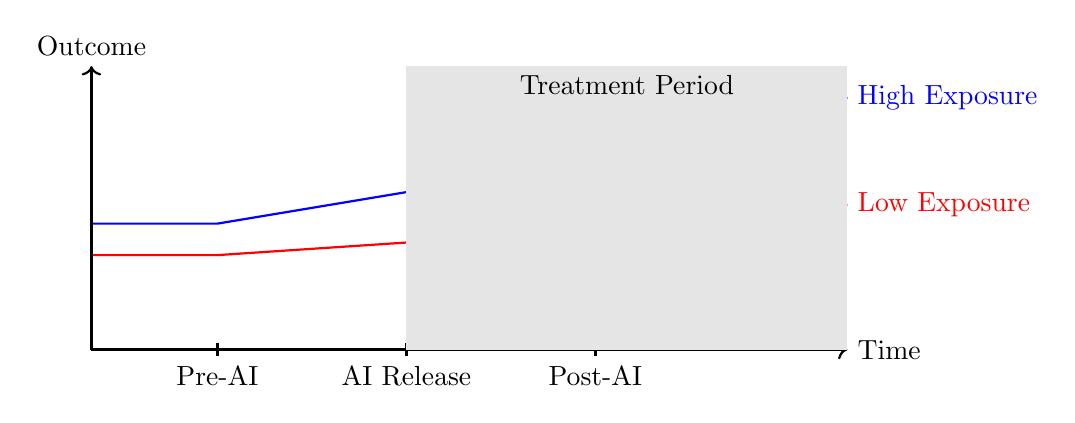
\begin{tikzpicture}[scale=0.8]
  % Timeline axis
  \draw[thick,->] (0,0) -- (12,0) node[right] {Time};
  % Event markers
  \foreach \x/\label in {2/Pre-AI,5/AI Release,8/Post-AI} {
    \draw[thick] (\x,0.1) -- (\x,-0.1) node[below,align=center] {\label};
  }
  % Treatment group line
  \draw[blue,thick] (0,2) -- (2,2) -- (5,2.5) -- (8,3.5) -- (12,4) node[right] {High Exposure};
  % Control group line  
  \draw[red,thick] (0,1.5) -- (2,1.5) -- (5,1.7) -- (8,2) -- (12,2.3) node[right] {Low Exposure};
  % Y-axis
  \draw[thick,->] (0,0) -- (0,4.5) node[above] {Outcome};
  % Shaded region for treatment period
  \fill[gray!20] (5,0) rectangle (12,4.5);
  \node at (8.5,4.2) {Treatment Period};
\end{tikzpicture}
\caption{Event-study timeline showing treatment and control groups around major AI release dates (GPT-3, GPT-4, etc.). The shaded region indicates the post-treatment period.}
\end{figure}

\begin{figure}[htbp]
\centering
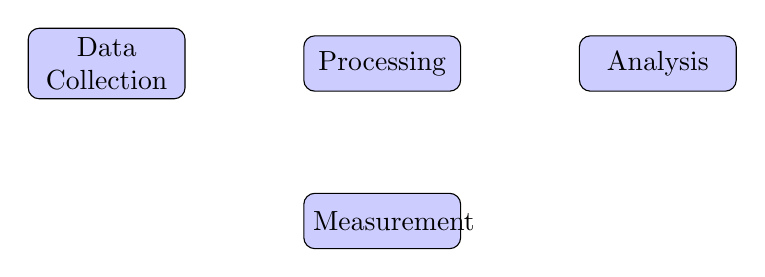
\begin{tikzpicture}[node distance=2cm,auto]
  \tikzstyle{block} = [rectangle, draw, fill=blue!20, text width=5em, text centered, rounded corners, minimum height=2em]
  \tikzstyle{arrow} = [thick,->,>=stealth]
  % Nodes
  \node [block] (data) {Data Collection};
  \node [block, right of=data, node distance=3.5cm] (process) {Processing};
  \node [block, right of=process, node distance=3.5cm] (analysis) {Analysis};
  \node [block, below of=process] (measure) {Measurement};
  % Arrows
  \path [arrow] (data) -- (process);
  \path [arrow] (process) -- (analysis);
  \path [arrow] (process) -- (measure);
\end{tikzpicture}
\caption{Data processing pipeline showing the flow from occupational databases through exposure measurement to asset pricing tests.}
\end{figure}

\bibliographystyle{plain}


\begin{thebibliography}{99}
\bibitem{Autor2003} A. Vaswani, N. Shazeer, N. Parmar, et al.. ``Attention is All You Need.'' Advances in Neural Information Processing Systems 30, 2017. doi:10.48550/arXiv.1706.03762.
\bibitem{AcemogluRestrepo2019} T. Brown, B. Mann, N. Ryder, et al.. ``Language Models are Few-Shot Learners.'' Advances in Neural Information Processing Systems 33, 2020. doi:10.48550/arXiv.2005.14165.
\end{thebibliography}
\end{document}